\documentclass[]{article}
\usepackage{lmodern}
\usepackage{amssymb,amsmath}
\usepackage{ifxetex,ifluatex}
\usepackage{fixltx2e} % provides \textsubscript
\ifnum 0\ifxetex 1\fi\ifluatex 1\fi=0 % if pdftex
  \usepackage[T1]{fontenc}
  \usepackage[utf8]{inputenc}
\else % if luatex or xelatex
  \ifxetex
    \usepackage{mathspec}
  \else
    \usepackage{fontspec}
  \fi
  \defaultfontfeatures{Ligatures=TeX,Scale=MatchLowercase}
  \newcommand{\euro}{€}
\fi
% use upquote if available, for straight quotes in verbatim environments
\IfFileExists{upquote.sty}{\usepackage{upquote}}{}
% use microtype if available
\IfFileExists{microtype.sty}{%
\usepackage{microtype}
\UseMicrotypeSet[protrusion]{basicmath} % disable protrusion for tt fonts
}{}
\usepackage[margin=1in]{geometry}
\usepackage{hyperref}
\PassOptionsToPackage{usenames,dvipsnames}{color} % color is loaded by hyperref
\hypersetup{unicode=true,
            pdftitle={Panel Data Models},
            pdfborder={0 0 0},
            breaklinks=true}
\urlstyle{same}  % don't use monospace font for urls
\usepackage{color}
\usepackage{fancyvrb}
\newcommand{\VerbBar}{|}
\newcommand{\VERB}{\Verb[commandchars=\\\{\}]}
\DefineVerbatimEnvironment{Highlighting}{Verbatim}{commandchars=\\\{\}}
% Add ',fontsize=\small' for more characters per line
\usepackage{framed}
\definecolor{shadecolor}{RGB}{248,248,248}
\newenvironment{Shaded}{\begin{snugshade}}{\end{snugshade}}
\newcommand{\KeywordTok}[1]{\textcolor[rgb]{0.13,0.29,0.53}{\textbf{{#1}}}}
\newcommand{\DataTypeTok}[1]{\textcolor[rgb]{0.13,0.29,0.53}{{#1}}}
\newcommand{\DecValTok}[1]{\textcolor[rgb]{0.00,0.00,0.81}{{#1}}}
\newcommand{\BaseNTok}[1]{\textcolor[rgb]{0.00,0.00,0.81}{{#1}}}
\newcommand{\FloatTok}[1]{\textcolor[rgb]{0.00,0.00,0.81}{{#1}}}
\newcommand{\ConstantTok}[1]{\textcolor[rgb]{0.00,0.00,0.00}{{#1}}}
\newcommand{\CharTok}[1]{\textcolor[rgb]{0.31,0.60,0.02}{{#1}}}
\newcommand{\SpecialCharTok}[1]{\textcolor[rgb]{0.00,0.00,0.00}{{#1}}}
\newcommand{\StringTok}[1]{\textcolor[rgb]{0.31,0.60,0.02}{{#1}}}
\newcommand{\VerbatimStringTok}[1]{\textcolor[rgb]{0.31,0.60,0.02}{{#1}}}
\newcommand{\SpecialStringTok}[1]{\textcolor[rgb]{0.31,0.60,0.02}{{#1}}}
\newcommand{\ImportTok}[1]{{#1}}
\newcommand{\CommentTok}[1]{\textcolor[rgb]{0.56,0.35,0.01}{\textit{{#1}}}}
\newcommand{\DocumentationTok}[1]{\textcolor[rgb]{0.56,0.35,0.01}{\textbf{\textit{{#1}}}}}
\newcommand{\AnnotationTok}[1]{\textcolor[rgb]{0.56,0.35,0.01}{\textbf{\textit{{#1}}}}}
\newcommand{\CommentVarTok}[1]{\textcolor[rgb]{0.56,0.35,0.01}{\textbf{\textit{{#1}}}}}
\newcommand{\OtherTok}[1]{\textcolor[rgb]{0.56,0.35,0.01}{{#1}}}
\newcommand{\FunctionTok}[1]{\textcolor[rgb]{0.00,0.00,0.00}{{#1}}}
\newcommand{\VariableTok}[1]{\textcolor[rgb]{0.00,0.00,0.00}{{#1}}}
\newcommand{\ControlFlowTok}[1]{\textcolor[rgb]{0.13,0.29,0.53}{\textbf{{#1}}}}
\newcommand{\OperatorTok}[1]{\textcolor[rgb]{0.81,0.36,0.00}{\textbf{{#1}}}}
\newcommand{\BuiltInTok}[1]{{#1}}
\newcommand{\ExtensionTok}[1]{{#1}}
\newcommand{\PreprocessorTok}[1]{\textcolor[rgb]{0.56,0.35,0.01}{\textit{{#1}}}}
\newcommand{\AttributeTok}[1]{\textcolor[rgb]{0.77,0.63,0.00}{{#1}}}
\newcommand{\RegionMarkerTok}[1]{{#1}}
\newcommand{\InformationTok}[1]{\textcolor[rgb]{0.56,0.35,0.01}{\textbf{\textit{{#1}}}}}
\newcommand{\WarningTok}[1]{\textcolor[rgb]{0.56,0.35,0.01}{\textbf{\textit{{#1}}}}}
\newcommand{\AlertTok}[1]{\textcolor[rgb]{0.94,0.16,0.16}{{#1}}}
\newcommand{\ErrorTok}[1]{\textcolor[rgb]{0.64,0.00,0.00}{\textbf{{#1}}}}
\newcommand{\NormalTok}[1]{{#1}}
\usepackage{longtable,booktabs}
\usepackage{graphicx,grffile}
\makeatletter
\def\maxwidth{\ifdim\Gin@nat@width>\linewidth\linewidth\else\Gin@nat@width\fi}
\def\maxheight{\ifdim\Gin@nat@height>\textheight\textheight\else\Gin@nat@height\fi}
\makeatother
% Scale images if necessary, so that they will not overflow the page
% margins by default, and it is still possible to overwrite the defaults
% using explicit options in \includegraphics[width, height, ...]{}
\setkeys{Gin}{width=\maxwidth,height=\maxheight,keepaspectratio}
\setlength{\parindent}{0pt}
\setlength{\parskip}{6pt plus 2pt minus 1pt}
\setlength{\emergencystretch}{3em}  % prevent overfull lines
\providecommand{\tightlist}{%
  \setlength{\itemsep}{0pt}\setlength{\parskip}{0pt}}
\setcounter{secnumdepth}{5}

%%% Use protect on footnotes to avoid problems with footnotes in titles
\let\rmarkdownfootnote\footnote%
\def\footnote{\protect\rmarkdownfootnote}

%%% Change title format to be more compact
\usepackage{titling}

% Create subtitle command for use in maketitle
\newcommand{\subtitle}[1]{
  \posttitle{
    \begin{center}\large#1\end{center}
    }
}

\setlength{\droptitle}{-2em}
  \title{Panel Data Models}
  \pretitle{\vspace{\droptitle}\centering\huge}
  \posttitle{\par}
  \author{}
  \preauthor{}\postauthor{}
  \date{}
  \predate{}\postdate{}


% Redefines (sub)paragraphs to behave more like sections
\ifx\paragraph\undefined\else
\let\oldparagraph\paragraph
\renewcommand{\paragraph}[1]{\oldparagraph{#1}\mbox{}}
\fi
\ifx\subparagraph\undefined\else
\let\oldsubparagraph\subparagraph
\renewcommand{\subparagraph}[1]{\oldsubparagraph{#1}\mbox{}}
\fi


\usepackage{amsthm}
\newtheorem{theorem}{Theorem}[section]
\newtheorem{lemma}{Lemma}[section]
\theoremstyle{definition}
\newtheorem{definition}{Definition}[section]
\newtheorem{corollary}{Corollary}[section]
\newtheorem{proposition}{Proposition}[section]
\theoremstyle{definition}
\newtheorem{example}{Example}[section]
\theoremstyle{remark}
\newtheorem*{remark}{Remark}
\begin{document}
\maketitle

{
\setcounter{tocdepth}{2}
\tableofcontents
}
\section{Introduction}\label{introduction}

This workshop will take a practical look at panel data methods and
models. Political scientists often approach research questions which
have important time and space implications. Policy makers might face
choices and questions of a similar nature: what effect does the building
of a polluting power plant have on house prices? Is education a helpful
tool to reduce the gender wage gap?

Panel data are useful to test hypotheses in these contexts, but come
with new methodological and substantive challenges. Together we will
look at these topics:

\begin{itemize}
\tightlist
\item
  Panel data, what does it look like? How do we describe our samples?
\item
  Adapting Ordinary Least Squares to estimate models using panel data
  (especially focusing on the challenges of controlling for unobserved
  heterogeneity, errors, and lagged variables)
\item
  Implementation of the models in R
\item
  Substantive interpretation of model results from a practical
  policy-making point of view.
\end{itemize}

\begin{center}\rule{0.5\linewidth}{\linethickness}\end{center}

\emph{Last Updated: May 25, 2017 10:58 AM}

\section{Acknowledgments}\label{acknowledgments}

The content of this workshop is based on the material from
\href{https://uclspp.github.io/PUBLG100}{Introduction to Quantitative
Methods} course at UCL.

This work is licensed under a Creative Commons Attribution-ShareAlike
4.0 International License.

\section{Panel Data Models}\label{panel-data-models}

\begin{itemize}
\item
  Panel data are datasets in which a set of units (for example people)
  are observed for several time periods.
\item
  If experimental data are not available, then the use of panel data is
  one important approach to reduce the problem of omitted variable bias.
\item
  There are many empirical research areas where results that are not
  based on panel data are no longer taken seriously.
\end{itemize}

\subsection{Fixed Effects Model}\label{fixed-effects-model}

\begin{itemize}
\item
  The fixed effects model is simply a variation on the linear regression
  model.
\item
  Its key advantage is that it enables us to control for all variables
  that vary over the cross-sectional units but are constant over time.
\end{itemize}

\subsubsection{Example: Traffic Fatalities and Beer
Tax}\label{example-traffic-fatalities-and-beer-tax}

Dataset from Stock \& Watson (Ch.10), covers state traffic fatality data
available for 48 states observed over seven years (from 1982 to 1988),
for a total of 336 observations.

\begin{tabular}{l|r|r|r|r|r|r|r|r}
\hline
state & year & mrall & beertax & mlda & jaild & vmiles & unrate & perinc\\
\hline
AL & 1982 & 0.0002128 & 1.5393795 & 19.00 & 0 & 7233.887 & 14.4 & 10544.15\\
\hline
AL & 1983 & 0.0002348 & 1.7889907 & 19.00 & 0 & 7836.348 & 13.7 & 10732.80\\
\hline
AL & 1984 & 0.0002336 & 1.7142856 & 19.00 & 0 & 8262.990 & 11.1 & 11108.79\\
\hline
AL & 1985 & 0.0002193 & 1.6525424 & 19.67 & 0 & 8726.917 & 8.9 & 11332.63\\
\hline
AL & 1986 & 0.0002669 & 1.6099070 & 21.00 & 0 & 8952.854 & 9.8 & 11661.51\\
\hline
AL & 1987 & 0.0002719 & 1.5599999 & 21.00 & 0 & 9166.302 & 7.8 & 11944.00\\
\hline
AL & 1988 & 0.0002494 & 1.5014436 & 21.00 & 0 & 9674.323 & 7.2 & 12368.62\\
\hline
AZ & 1982 & 0.0002499 & 0.2147971 & 19.00 & 1 & 6810.157 & 9.9 & 12309.07\\
\hline
AZ & 1983 & 0.0002267 & 0.2064220 & 19.00 & 1 & 6587.495 & 9.1 & 12693.81\\
\hline
AZ & 1984 & 0.0002829 & 0.2967033 & 19.00 & 1 & 6709.970 & 5.0 & 13265.93\\
\hline
\end{tabular}

\subsection{Assumptions of the Fixed Effects
Model}\label{assumptions-of-the-fixed-effects-model}

\begin{itemize}
\item
  The fixed effects model assumes that the true relationship is:

  \[\begin{aligned}
  y_{i,t} = \beta_0 + \beta_1x_{i,t} + \beta_2z_i + u_{i,t} \end{aligned}\]

  where in the S\&W example \(y_{i,t}\) would be the number of traffic
  fatalities and \(x_{i,t}\) the beer tax in state \(i\) in year \(t\).
\item
  Note that the variable \(z_i\) does not have a time index and is
  therefore assumed to be constant over time.
\item
  In this example \(z_i\) could be the social attitude towards drunk
  driving in state \(i\).
\item
  If we define \(\alpha_i = \beta_0 + \beta_2z_i\), then (1) simplifies
  to

  \[\begin{aligned}
  y_{i,t} = \alpha_i + \beta_1x_{i,t} + u_{i,t} \end{aligned}\]
\item
  The graphical interpretation of \(\alpha_i\) is that it is the
  intercept of the relationship between alcohol taxes and traffic
  fatalities in state \(i\).
\item
  It is straightforward to allow for further variables which are
  constant over time in (1).
\item
  In this case the intercepts \(\alpha_i\) reflect the combined effect
  of several variables which are constant over time.
\end{itemize}

\begin{figure}[htbp]
\centering
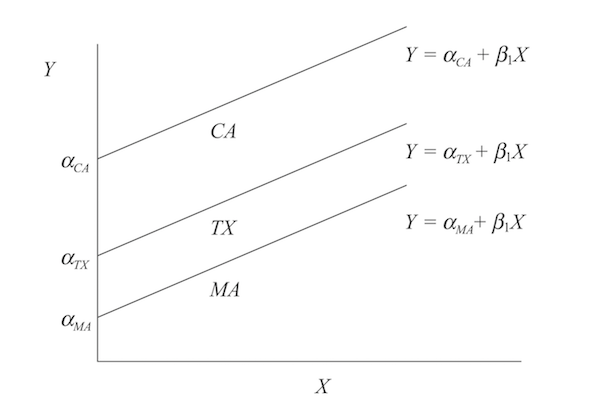
\includegraphics{./img/fixed_effects.png}
\caption{}
\end{figure}

\subsection{Advantages and
Disadvantages}\label{advantages-and-disadvantages}

\begin{itemize}
\item
  The key advantage of the fixed effects model is that it allows us to
  control for all time invariant omitted variables.
\item
  This is particularly important in the case of variables which are
  difficult or impossible to observe.
\item
  The key disadvantage is that we have to estimate a number of
  additional parameters.
\item
  Furthermore, it will be impossible to estimate the effect of variables
  which do not (or hardly) vary over time.
\end{itemize}

\subsection{Time Fixed Effects}\label{time-fixed-effects}

\begin{itemize}
\item
  The basic fixed effects model only prevents omitted variable bias from
  variables that do not change over time.
\item
  However, panel data allow us to control also for omitted variable bias
  from one other type of omitted variable.
\item
  In the traffic fatalities example technical progress could be an
  important determinant of the number of deaths and could also be
  correlated with alcohol taxes.
\item
  At the same time this variable probably affects all states in the same
  way (i.e.~does not vary across states).
\end{itemize}

\subsection{Time and Unit Fixed
Effects}\label{time-and-unit-fixed-effects}

\begin{itemize}
\item
  In most applications we use both unit and time fixed effects at the
  same time.
\item
  This model is sometimes referred to as the ``twoway fixed effects''
  model.
\item
  In the literature the cross-sectional fixed effects are referred to as
  ``fixed effects'', ``state (fixed) effects'', ``firm (fixed) effects''
  or ``person (fixed) effects''.
\item
  Similarly, time fixed effects are often referred to as ``time
  effects''.
\end{itemize}

\section{Violations of Assumptions}\label{violations-of-assumptions}

\subsection{Assumption 2 in Panel
Data}\label{assumption-2-in-panel-data}

\begin{itemize}
\item
  Panel data is characterized by time dependency for each panel unit.
\item
  As discussed in Week 6, this is a violation of the regression
  Assumption 2 (X and Y are i.i.d).
\end{itemize}

\subsubsection{Serial Correlation}\label{serial-correlation}

\begin{itemize}
\item
  Time dependency is often described as autocorrelation or serial
  correlation.
\item
  The main approach to deal with serial correlation is by adjusting
  standard errors to take into account autocorrelation.
\item
  If there is substantial autocorrelation (serial correlation) in the
  error term, even heteroskedasticity-robust standard errors will be
  inconsistent.
\item
  In panel data as in any other time series data, autocorrelation can be
  a very serious concern.
\item
  We can test for serial correlation after our fixed effects estimation
  using the Breusch-Godfrey test.
\item
  The null hypothesis in this test is that the autocorrelation of the
  error term is 0.
\end{itemize}

\subsubsection{Cross-sectional
dependence}\label{cross-sectional-dependence}

\begin{itemize}
\item
  Cross-sectional dependence in panels may arise when e.g.~countries
  respond to common shocks or if spatial diffusion processes are present
  (think Arab Spring, or shocks from the financial crisis).
\item
  If cross-sectional dependence is present, this results, at least, in
  the inefficiency of the estimators and invalid inference when using
  standard estimation techniques.
\item
  This is another instance of the violation of regression Assumption 2.
\item
  If we assume that our earlier two-way fixed effects model
  specification is consistent, then we can test for residual
  cross-sectional dependence after the introduction of two-way fixed
  effects to account for common shocks.
\end{itemize}

\subsection{Panel-corrected Standard
Errors}\label{panel-corrected-standard-errors}

\begin{itemize}
\item
  Panel-corrected standard errors (Beck and Katz 1995)

  \begin{itemize}
  \item
    \textbf{panel heteroskedasticity}: each country may have its own
    error variance
  \item
    \textbf{contemporaneous correlation of the errors}: the error for
    one country may be correlated with the errors for other countries in
    the same year
  \item
    \textbf{serially correlated errors}: the errors for a given country
    are correlated with previous errors for that country
  \end{itemize}
\end{itemize}

\subsection{General Approach to Correlation Between
Panels}\label{general-approach-to-correlation-between-panels}

\begin{itemize}
\item
  Driscoll and Kraay (1998) propose an estimator producing
  heteroskedasticity- and autocorrelation- consistent standard errors
  that are robust to general forms of spatial and temporal dependence.
  Often known as the SCC estimator.
\item
  Panel Corrected Standard Errors (PCSE), while popular in political
  science, may not work well with shorter panels with large N (ratio of
  T/N is small).
\item
  SCC estimator performs equally well in large N settings.
\end{itemize}

\subsection{Your Roadmap with Panel
Data}\label{your-roadmap-with-panel-data}

\begin{itemize}
\item
  Is it a fixed effects or random effects model?
\item
  Hausman test. But primarily the choice should be driven by theory!
\item
  Use robust standard errors, start with HAC.
\item
  Check whether there is any cross-sectional dependence:
\item
  If not, you can stick to HAC.
\item
  If you have cross-sectional dependence, you need to use PCSE or SCC
  (use SCC).
\end{itemize}

\section{Hands-on Tutorial}\label{hands-on-tutorial}

Let's start by load these packages:

\begin{Shaded}
\begin{Highlighting}[]
\KeywordTok{library}\NormalTok{(plm)}
\KeywordTok{library}\NormalTok{(lmtest)}
\KeywordTok{library}\NormalTok{(texreg)}
\end{Highlighting}
\end{Shaded}

Clear the environment

\begin{Shaded}
\begin{Highlighting}[]
\KeywordTok{rm}\NormalTok{(}\DataTypeTok{list =} \KeywordTok{ls}\NormalTok{())}
\end{Highlighting}
\end{Shaded}

\subsection{More Guns, Less Crimes}\label{more-guns-less-crimes}

Download the guns dataset used by Stock and Watson.

\begin{itemize}
\tightlist
\item
  \textbf{\href{http://uclspp.github.io/PUBLG100/data/guns.csv}{Dataset}}
\item
  \textbf{\href{http://wps.aw.com/wps/media/objects/11422/11696965/data3eu/Guns_Description.pdf}{Codebook}}
\end{itemize}

Gun rights advocate John Lott argues in his book
\href{https://en.wikipedia.org/wiki/More_Guns,_Less_Crime}{More Guns,
Less Crimes} that crime rates in the United States decrease when gun
ownership restrictions are relaxed. The data used in Lott's research
compares violent crimes, robberies, and murders across 50 states to
determine whether the so called ``shall'' laws that remove discretion
from license granting authorities actually decrease crime rates. So far
41 states have passed these ``shall'' laws where a person applying for a
licence to carry a concealed weapon doesn't have to provide
justification or ``good cause'' for requiring a concealed weapon permit.

Let's load the dataset used by Lott and see if we can test the arguments
made by gun rights advocates.

\begin{Shaded}
\begin{Highlighting}[]
\NormalTok{guns <-}\StringTok{ }\KeywordTok{read.csv}\NormalTok{(}\StringTok{"guns.csv"}\NormalTok{)}
\end{Highlighting}
\end{Shaded}

The variables we're interested in are described below.

\begin{longtable}[c]{@{}ll@{}}
\toprule
\begin{minipage}[b]{0.17\columnwidth}\raggedright\strut
Variable
\strut\end{minipage} &
\begin{minipage}[b]{0.74\columnwidth}\raggedright\strut
Definition
\strut\end{minipage}\tabularnewline
\midrule
\endhead
\begin{minipage}[t]{0.17\columnwidth}\raggedright\strut
mur
\strut\end{minipage} &
\begin{minipage}[t]{0.74\columnwidth}\raggedright\strut
Murder rate (incidents per 100,000)
\strut\end{minipage}\tabularnewline
\begin{minipage}[t]{0.17\columnwidth}\raggedright\strut
shall
\strut\end{minipage} &
\begin{minipage}[t]{0.74\columnwidth}\raggedright\strut
= 1 if the state has a shall-carry law in effect in that year = 0
otherwise
\strut\end{minipage}\tabularnewline
\begin{minipage}[t]{0.17\columnwidth}\raggedright\strut
incarc\_rate
\strut\end{minipage} &
\begin{minipage}[t]{0.74\columnwidth}\raggedright\strut
Incarceration rate in the state in the previous year (sentenced
prisoners per 100,000 residents; value for the previous year)
\strut\end{minipage}\tabularnewline
\begin{minipage}[t]{0.17\columnwidth}\raggedright\strut
pm1029
\strut\end{minipage} &
\begin{minipage}[t]{0.74\columnwidth}\raggedright\strut
Percent of state population that is male, ages 10 to 29
\strut\end{minipage}\tabularnewline
\begin{minipage}[t]{0.17\columnwidth}\raggedright\strut
stateid
\strut\end{minipage} &
\begin{minipage}[t]{0.74\columnwidth}\raggedright\strut
ID number of states (Alabama = 1, Alaska = 2, etc.)
\strut\end{minipage}\tabularnewline
\begin{minipage}[t]{0.17\columnwidth}\raggedright\strut
year
\strut\end{minipage} &
\begin{minipage}[t]{0.74\columnwidth}\raggedright\strut
Year (1977-1999)
\strut\end{minipage}\tabularnewline
\bottomrule
\end{longtable}

We will focus on murder rates in this example but you could try the same
with variables measuring violent crimes or robberies as well.

Let's create a factor variable representing whether a state has passed
``shall'' law or not. The variable already exists as \texttt{0} or
\texttt{1} but we want to convert it to a factor for our analysis.

\begin{Shaded}
\begin{Highlighting}[]
\NormalTok{guns$shall <-}\StringTok{ }\KeywordTok{factor}\NormalTok{(guns$shall, }\DataTypeTok{levels =} \KeywordTok{c}\NormalTok{(}\DecValTok{0}\NormalTok{, }\DecValTok{1}\NormalTok{), }\DataTypeTok{labels =}\KeywordTok{c}\NormalTok{(}\StringTok{"NO"}\NormalTok{, }\StringTok{"YES"}\NormalTok{))}
\end{Highlighting}
\end{Shaded}

\subsection{Fixed Effects}\label{fixed-effects}

Let's estimate a fixed effect model on panel data using the
\texttt{plm()} function with \texttt{shall}, \texttt{incarc\_rate}, and
\texttt{pm1029} as the independent variables.

\begin{Shaded}
\begin{Highlighting}[]
\NormalTok{state_effects <-}\StringTok{ }\KeywordTok{plm}\NormalTok{(mur ~}\StringTok{ }\NormalTok{shall +}\StringTok{ }\NormalTok{incarc_rate +}\StringTok{ }\NormalTok{pm1029, }
                     \DataTypeTok{data =} \NormalTok{guns, }
                     \DataTypeTok{index =} \KeywordTok{c}\NormalTok{(}\StringTok{"stateid"}\NormalTok{, }\StringTok{"year"}\NormalTok{), }
                     \DataTypeTok{model =} \StringTok{"within"}\NormalTok{, }
                     \DataTypeTok{effect =} \StringTok{"individual"}\NormalTok{)}

\KeywordTok{summary}\NormalTok{(state_effects)}
\end{Highlighting}
\end{Shaded}

\begin{verbatim}
## Oneway (individual) effect Within Model
## 
## Call:
## plm(formula = mur ~ shall + incarc_rate + pm1029, data = guns, 
##     effect = "individual", model = "within", index = c("stateid", 
##         "year"))
## 
## Balanced Panel: n=51, T=23, N=1173
## 
## Residuals :
##       Min.    1st Qu.     Median    3rd Qu.       Max. 
## -21.102428  -0.958945   0.016047   1.082008  29.031961 
## 
## Coefficients :
##               Estimate Std. Error t-value  Pr(>|t|)    
## shallYES    -1.4513886  0.3154300 -4.6013 4.678e-06 ***
## incarc_rate  0.0174551  0.0011261 15.4998 < 2.2e-16 ***
## pm1029       0.9582993  0.0859610 11.1481 < 2.2e-16 ***
## ---
## Signif. codes:  0 '***' 0.001 '**' 0.01 '*' 0.05 '.' 0.1 ' ' 1
## 
## Total Sum of Squares:    12016
## Residual Sum of Squares: 9800
## R-Squared:      0.18444
## Adj. R-Squared: 0.14581
## F-statistic: 84.3526 on 3 and 1119 DF, p-value: < 2.22e-16
\end{verbatim}

The \texttt{state\_effects} model shows that all three of our
independent variables are statistically significant, with \texttt{shall}
decreasing murder rates by \texttt{1.45} incidents per \texttt{100000}
members of the population. The effects of incarceration rate and
percentage of male population between \texttt{10} and \texttt{29} years
old are also statistically significant.

Before drawing any conclusions let's make sure whether there are any
state effects in our model using
\href{http://bit.ly/r_plmtest}{\texttt{plmtest()}}.

\begin{Shaded}
\begin{Highlighting}[]
\KeywordTok{plmtest}\NormalTok{(state_effects, }\DataTypeTok{effect=}\StringTok{"individual"}\NormalTok{)}
\end{Highlighting}
\end{Shaded}

\begin{verbatim}
## 
##  Lagrange Multiplier Test - (Honda) for balanced panels
## 
## data:  mur ~ shall + incarc_rate + pm1029
## normal = 47.242, p-value < 2.2e-16
## alternative hypothesis: significant effects
\end{verbatim}

The p-value suggests the presence of state effects. In addition to state
fixed effects, a number of factors could affect the murder rate that are
not specific to an individual state. We can model these time fixed
effects using the \texttt{effect\ =\ "time"} argument in
\href{http://bit.ly/r_plm}{\texttt{plm()}}.

\begin{Shaded}
\begin{Highlighting}[]
\NormalTok{time_effects <-}\StringTok{ }\KeywordTok{plm}\NormalTok{(mur ~}\StringTok{ }\NormalTok{shall +}\StringTok{ }\NormalTok{incarc_rate +}\StringTok{ }\NormalTok{pm1029, }
                    \DataTypeTok{data =} \NormalTok{guns, }
                    \DataTypeTok{index =} \KeywordTok{c}\NormalTok{(}\StringTok{"stateid"}\NormalTok{, }\StringTok{"year"}\NormalTok{), }
                    \DataTypeTok{model =} \StringTok{"within"}\NormalTok{, }
                    \DataTypeTok{effect =} \StringTok{"time"}\NormalTok{)}

\KeywordTok{summary}\NormalTok{(time_effects)}
\end{Highlighting}
\end{Shaded}

\begin{verbatim}
## Oneway (time) effect Within Model
## 
## Call:
## plm(formula = mur ~ shall + incarc_rate + pm1029, data = guns, 
##     effect = "time", model = "within", index = c("stateid", "year"))
## 
## Balanced Panel: n=51, T=23, N=1173
## 
## Residuals :
##      Min.   1st Qu.    Median   3rd Qu.      Max. 
## -21.68350  -2.04596  -0.31955   1.76758  35.20084 
## 
## Coefficients :
##               Estimate Std. Error t-value Pr(>|t|)    
## shallYES    -0.2521605  0.3032163 -0.8316   0.4058    
## incarc_rate  0.0412157  0.0007704 53.4993   <2e-16 ***
## pm1029       0.2148597  0.1407613  1.5264   0.1272    
## ---
## Signif. codes:  0 '***' 0.001 '**' 0.01 '*' 0.05 '.' 0.1 ' ' 1
## 
## Total Sum of Squares:    65571
## Residual Sum of Squares: 18141
## R-Squared:      0.72334
## Adj. R-Squared: 0.71731
## F-statistic: 999.623 on 3 and 1147 DF, p-value: < 2.22e-16
\end{verbatim}

The \texttt{incarc\_rate} variable is the only statistically significant
variable in the time fixed effects model.

Now let's run \texttt{plmtest} on the \texttt{time\_effects} model to
verify if time fixed effects are indeed present in the model.

\begin{Shaded}
\begin{Highlighting}[]
\KeywordTok{plmtest}\NormalTok{(time_effects, }\DataTypeTok{effect=}\StringTok{"time"}\NormalTok{)}
\end{Highlighting}
\end{Shaded}

\begin{verbatim}
## 
##  Lagrange Multiplier Test - time effects (Honda) for balanced
##  panels
## 
## data:  mur ~ shall + incarc_rate + pm1029
## normal = 16.104, p-value < 2.2e-16
## alternative hypothesis: significant effects
\end{verbatim}

The \emph{p-value} tells us that we can reject the null hypothesis so we
know that there are time fixed effects present in our model.

We already confirmed the presence of state fixed effects in the first
model we estimated. Now, in order to control for both state AND time
fixed effects, we need to estimate a model using the
\texttt{effect\ =\ "twoways"} argument.

\begin{Shaded}
\begin{Highlighting}[]
\NormalTok{twoway_effects <-}\StringTok{ }\KeywordTok{plm}\NormalTok{(mur ~}\StringTok{ }\NormalTok{shall +}\StringTok{ }\NormalTok{incarc_rate +}\StringTok{ }\NormalTok{pm1029, }
                      \DataTypeTok{data =} \NormalTok{guns, }
                      \DataTypeTok{index =} \KeywordTok{c}\NormalTok{(}\StringTok{"stateid"}\NormalTok{, }\StringTok{"year"}\NormalTok{), }
                      \DataTypeTok{model =} \StringTok{"within"}\NormalTok{, }
                      \DataTypeTok{effect =} \StringTok{"twoways"}\NormalTok{)}

\KeywordTok{summary}\NormalTok{(twoway_effects)}
\end{Highlighting}
\end{Shaded}

\begin{verbatim}
## Twoways effects Within Model
## 
## Call:
## plm(formula = mur ~ shall + incarc_rate + pm1029, data = guns, 
##     effect = "twoways", model = "within", index = c("stateid", 
##         "year"))
## 
## Balanced Panel: n=51, T=23, N=1173
## 
## Residuals :
##        Min.     1st Qu.      Median     3rd Qu.        Max. 
## -19.2097691  -0.9748749  -0.0069663   1.0119176  27.1354552 
## 
## Coefficients :
##               Estimate Std. Error t-value  Pr(>|t|)    
## shallYES    -0.5640474  0.3325054 -1.6964 0.0901023 .  
## incarc_rate  0.0209756  0.0011252 18.6411 < 2.2e-16 ***
## pm1029       0.7326357  0.2189770  3.3457 0.0008485 ***
## ---
## Signif. codes:  0 '***' 0.001 '**' 0.01 '*' 0.05 '.' 0.1 ' ' 1
## 
## Total Sum of Squares:    11263
## Residual Sum of Squares: 8519.4
## R-Squared:      0.24357
## Adj. R-Squared: 0.19186
## F-statistic: 117.746 on 3 and 1097 DF, p-value: < 2.22e-16
\end{verbatim}

In a twoway fixed effects model \texttt{shall} is no longer significant
and the effect of male population between \texttt{10} and \texttt{29}
years old has decreased from \texttt{0.95} to \texttt{0.73} incidents
per \texttt{100,000} population.

The results of all three models are shown below.

\begin{Shaded}
\begin{Highlighting}[]
\KeywordTok{screenreg}\NormalTok{(}\KeywordTok{list}\NormalTok{(state_effects, time_effects, twoway_effects), }
          \DataTypeTok{custom.model.names =} \KeywordTok{c}\NormalTok{(}\StringTok{"State Fixed Effects"}\NormalTok{, }
                                 \StringTok{"Time Fixed Effects"}\NormalTok{, }
                                 \StringTok{"Twoway Fixed Effects"}\NormalTok{))}
\end{Highlighting}
\end{Shaded}

\begin{verbatim}
## 
## ==========================================================================
##              State Fixed Effects  Time Fixed Effects  Twoway Fixed Effects
## --------------------------------------------------------------------------
## shallYES       -1.45 ***            -0.25               -0.56             
##                (0.32)               (0.30)              (0.33)            
## incarc_rate     0.02 ***             0.04 ***            0.02 ***         
##                (0.00)               (0.00)              (0.00)            
## pm1029          0.96 ***             0.21                0.73 ***         
##                (0.09)               (0.14)              (0.22)            
## --------------------------------------------------------------------------
## R^2             0.18                 0.72                0.24             
## Adj. R^2        0.15                 0.72                0.19             
## Num. obs.    1173                 1173                1173                
## ==========================================================================
## *** p < 0.001, ** p < 0.01, * p < 0.05
\end{verbatim}

\subsection{Serial Correlation}\label{serial-correlation-1}

For time series data we need to address the potential for serial
correlation in the error term. We will test for serial correlation with
Breusch-Godfrey test using \texttt{pbgtest()} and provide solutions for
correcting it if necessary.

\begin{Shaded}
\begin{Highlighting}[]
\KeywordTok{pbgtest}\NormalTok{(twoway_effects)}
\end{Highlighting}
\end{Shaded}

\begin{verbatim}
## 
##  Breusch-Godfrey/Wooldridge test for serial correlation in panel
##  models
## 
## data:  mur ~ shall + incarc_rate + pm1029
## chisq = 765.16, df = 23, p-value < 2.2e-16
## alternative hypothesis: serial correlation in idiosyncratic errors
\end{verbatim}

The null hypothesis for the Breusch-Godfrey test is that there is no
serial correlation. The \texttt{p-value} from the test tells us that we
can reject the null hypothesis and confirms the presence of serial
correlation in our error term.

We can correct for serial correlation using
\href{http://bit.ly/r_coeftest}{\texttt{coeftest()}} similar to how we
corrected for heteroskedastic errors. We'll use the
\href{http://bit.ly/r_vcovHC}{\texttt{vcovHC()}} function for obtaining
a heteroskedasticity-consistent covariance matrix, but since we're
interested in correcting for autocorrelation as well, we will specify
\texttt{method\ =\ "arellano"} which corrects for both
heteroskedasticity and autocorrelation.

\begin{Shaded}
\begin{Highlighting}[]
\NormalTok{twoway_effects_hac <-}\StringTok{ }\KeywordTok{coeftest}\NormalTok{(twoway_effects, }
                               \DataTypeTok{vcov =} \KeywordTok{vcovHC}\NormalTok{(twoway_effects, }
                                             \DataTypeTok{method =} \StringTok{"arellano"}\NormalTok{, }
                                             \DataTypeTok{type =} \StringTok{"HC3"}\NormalTok{))}

\KeywordTok{screenreg}\NormalTok{(}\KeywordTok{list}\NormalTok{(twoway_effects, twoway_effects_hac),}
          \DataTypeTok{custom.model.names =} \KeywordTok{c}\NormalTok{(}\StringTok{"Twoway Fixed Effects"}\NormalTok{, }
                                 \StringTok{"Twoway Fixed Effects (HAC)"}\NormalTok{))}
\end{Highlighting}
\end{Shaded}

\begin{verbatim}
## 
## =============================================================
##              Twoway Fixed Effects  Twoway Fixed Effects (HAC)
## -------------------------------------------------------------
## shallYES       -0.56               -0.56                     
##                (0.33)              (0.48)                    
## incarc_rate     0.02 ***            0.02 *                   
##                (0.00)              (0.01)                    
## pm1029          0.73 ***            0.73                     
##                (0.22)              (0.54)                    
## -------------------------------------------------------------
## R^2             0.24                                         
## Adj. R^2        0.19                                         
## Num. obs.    1173                                            
## =============================================================
## *** p < 0.001, ** p < 0.01, * p < 0.05
\end{verbatim}

We can see that with heteroskedasticity and autocorrelation consistent
(HAC) standard errors, the percent of male population (10 - 29 yr old)
is no longer a significant predictor in our model.

\subsection{Cross-sectional
Dependence}\label{cross-sectional-dependence-1}

If a federal law imposed restrictions on gun ownership or licensing
requirements then the changes would likely affect all 50 states. This is
an example of Cross Sectional Dependence and not accounted for in a
fixed effect model. Other scenarios could also trigger cross sectional
dependence that we should take into consideration. For example, security
policies and law enforcement efforts might change after an extraordinary
event (think of mass shootings or terrorist attacks) thus influencing
law enforcement practices in all states. We can check for cross
sectional dependence using the Pesaran cross sectional dependence test
or \href{http://bit.ly/r_pcdtest}{\texttt{pcdtest()}}.

\begin{Shaded}
\begin{Highlighting}[]
\KeywordTok{pcdtest}\NormalTok{(twoway_effects)}
\end{Highlighting}
\end{Shaded}

\begin{verbatim}
## 
##  Pesaran CD test for cross-sectional dependence in panels
## 
## data:  mur ~ shall + incarc_rate + pm1029
## z = 3.9121, p-value = 9.148e-05
## alternative hypothesis: cross-sectional dependence
\end{verbatim}

As we've seen with other tests, the null hypothesis is that there is no
cross sectional dependence. The p-value, however tells that there is
indeed cross-sectional dependence and we need to correct it. There are
two general approaches to correcting for cross sectional dependence.

\textbf{Beck and Katz (1995) method or Panel Corrected Standard Errors
(PCSE)}: We can obtain Panel Corrected Standard Errors (PCSE) by first
obtaining a robust variance-covariance matrix for panel models with the
Beck and Katz (1995) method using the
\href{(http://bit.ly/r_vcovBK)}{\texttt{vcovBK()}} and passing it to the
familiar \href{http://bit.ly/r_coeftest}{\texttt{coeftest()}} function.

\begin{Shaded}
\begin{Highlighting}[]
\NormalTok{twoway_effects_pcse <-}\StringTok{ }\KeywordTok{coeftest}\NormalTok{(twoway_effects, }
                                \DataTypeTok{vcov =} \KeywordTok{vcovBK}\NormalTok{(twoway_effects, }
                                              \DataTypeTok{type=}\StringTok{"HC3"}\NormalTok{, }
                                              \DataTypeTok{cluster =} \StringTok{"group"}\NormalTok{)) }

\NormalTok{twoway_effects_pcse}
\end{Highlighting}
\end{Shaded}

\begin{verbatim}
## 
## t test of coefficients:
## 
##               Estimate Std. Error t value  Pr(>|t|)    
## shallYES    -0.5640474  0.7662556 -0.7361    0.4618    
## incarc_rate  0.0209756  0.0028249  7.4253 2.254e-13 ***
## pm1029       0.7326357  0.5118496  1.4313    0.1526    
## ---
## Signif. codes:  0 '***' 0.001 '**' 0.01 '*' 0.05 '.' 0.1 ' ' 1
\end{verbatim}

The results from PCSE are sensitive to the ratio between the number of
time periods in the dataset (T) and the total number of observations
(N). When we're dealing with large datasets (i.e.~the T/N ratio is
small), we use the Driscoll and Kraay method instead.

\textbf{Driscoll and Kraay (1998) (SCC)}: The cross-sectional and serial
correlation (SCC) method by Driscoll and Kraay addresses the limitations
of Beck and Katz's PCSE method is therefore preferred for obtaining
heteroskedasticity and autocorrelation consistent errors that are also
robust to cross-sectional dependence. We can get SCC corrected
covariance matrix using the
\href{http://bit.ly/r_vcovSCC}{\texttt{vcovSCC()}} function.

\begin{Shaded}
\begin{Highlighting}[]
\NormalTok{twoway_effects_scc <-}\StringTok{ }\KeywordTok{coeftest}\NormalTok{(twoway_effects,}
                               \DataTypeTok{vcov =} \KeywordTok{vcovSCC}\NormalTok{(twoway_effects, }
                                              \DataTypeTok{type=}\StringTok{"HC3"}\NormalTok{, }
                                              \DataTypeTok{cluster =} \StringTok{"group"}\NormalTok{))}

\NormalTok{twoway_effects_scc}
\end{Highlighting}
\end{Shaded}

\begin{verbatim}
## 
## t test of coefficients:
## 
##              Estimate Std. Error t value Pr(>|t|)  
## shallYES    -0.564047   0.542698 -1.0393  0.29888  
## incarc_rate  0.020976   0.010321  2.0324  0.04236 *
## pm1029       0.732636   0.551066  1.3295  0.18396  
## ---
## Signif. codes:  0 '***' 0.001 '**' 0.01 '*' 0.05 '.' 0.1 ' ' 1
\end{verbatim}

\begin{Shaded}
\begin{Highlighting}[]
\KeywordTok{screenreg}\NormalTok{(}\KeywordTok{list}\NormalTok{(state_effects, }
               \NormalTok{time_effects, }
               \NormalTok{twoway_effects, }
               \NormalTok{twoway_effects_pcse, }
               \NormalTok{twoway_effects_scc), }
          \DataTypeTok{custom.model.names =} \KeywordTok{c}\NormalTok{(}\StringTok{"State Effects"}\NormalTok{, }
                                 \StringTok{"Time Effects"}\NormalTok{, }
                                 \StringTok{"Twoway Fixed Effects"}\NormalTok{, }
                                 \StringTok{"PCSE"}\NormalTok{, }
                                 \StringTok{"SCC"}\NormalTok{))}
\end{Highlighting}
\end{Shaded}

\begin{verbatim}
## 
## ==================================================================================
##              State Effects  Time Effects  Twoway Fixed Effects  PCSE       SCC    
## ----------------------------------------------------------------------------------
## shallYES       -1.45 ***      -0.25         -0.56               -0.56      -0.56  
##                (0.32)         (0.30)        (0.33)              (0.77)     (0.54) 
## incarc_rate     0.02 ***       0.04 ***      0.02 ***            0.02 ***   0.02 *
##                (0.00)         (0.00)        (0.00)              (0.00)     (0.01) 
## pm1029          0.96 ***       0.21          0.73 ***            0.73       0.73  
##                (0.09)         (0.14)        (0.22)              (0.51)     (0.55) 
## ----------------------------------------------------------------------------------
## R^2             0.18           0.72          0.24                                 
## Adj. R^2        0.15           0.72          0.19                                 
## Num. obs.    1173           1173          1173                                    
## ==================================================================================
## *** p < 0.001, ** p < 0.01, * p < 0.05
\end{verbatim}

\section{Exercises}\label{exercises}

Download the traffic fatality dataset used in Stock and Watson examples.
It covers data from 48 states observed over seven years (from 1982 to
1988), for a total of 336 observations.

\begin{itemize}
\tightlist
\item
  \textbf{\href{https://altaf-ali.github.io/panel_data_models/data/fatality.dta}{Dataset}}
\end{itemize}

\begin{longtable}[c]{@{}ll@{}}
\toprule
Variable & Description\tabularnewline
\midrule
\endhead
mrall & Vehicle Fatality Rate (VFR)\tabularnewline
beertax & Tax on Case of Beer\tabularnewline
mlda & Minimum Legal Drinking Age\tabularnewline
jaild & Mandatory Jail Sentence\tabularnewline
vmiles & Average Mile per Driver\tabularnewline
unrate & Unemployment Rate\tabularnewline
perinc & Per Capita Personal Income\tabularnewline
\bottomrule
\end{longtable}

\begin{enumerate}
\def\labelenumi{\arabic{enumi}.}
\tightlist
\item
  Estimate a model for Vehicle Fatality Rate using your choice of
  variables listed above.

  \begin{itemize}
  \tightlist
  \item
    Estimate a fixed effect model and test for state and time fixed
    effects.
  \item
    Run the necessary tests to check whether state and time fixed
    effects are present.
  \end{itemize}
\item
  Estimate a twoway model and compare to the previous state and time
  fixed effect models.
\item
  Test for serial correlation and cross sectional dependence in the
  twoway model.
\item
  If either serial correlation or cross sectional dependence is present,
  use the methods you've learned to obtain heteroskedastic and
  autocorrelation consistent standard errors.
\item
  Compare the HAC and spatially robust standard errors with the twoway
  model estimated earlier.
\item
  Display the results in publication-ready tables and discuss the
  substantively significant findings.
\end{enumerate}

\end{document}
